
% \subsection{INSTITUTIONAL SHIFTS AND STRUCTURES}
\subsection{分水制度与流域SES构件的演变}\label{results-1}

\begin{figure}[!t]
	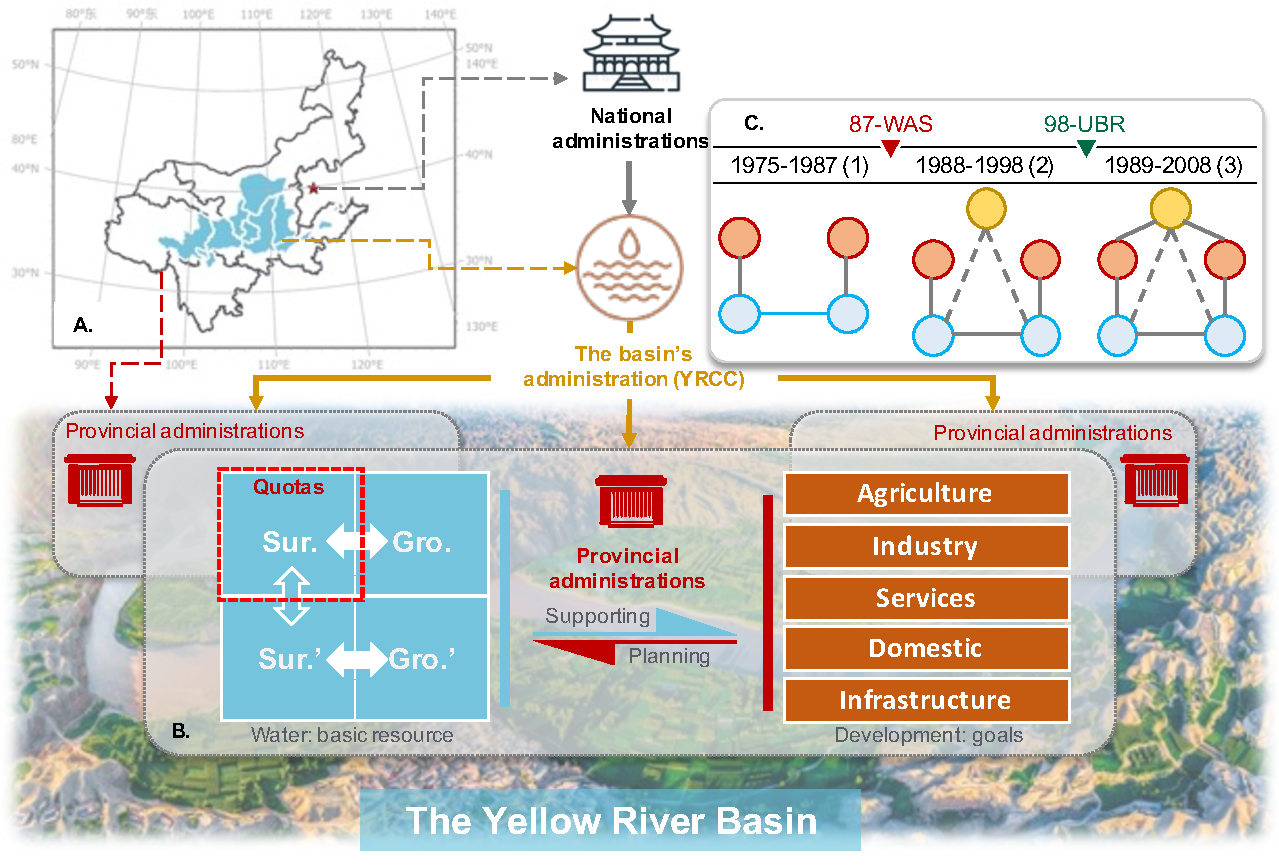
\includegraphics[width=\linewidth]{img/ch5/diagram.pdf}
	\caption[黄河流域社会经济制度变迁及其结构]{
		黄河流域社会经济制度变迁及其结构。
		\textbf{A.} 黄河流域跨越$10$个省(地区),其中$8$个对黄河流域水资源的依赖程度较高。国家部委(水利部)是发布水治理政策的最高权力机构,这些政策通常由流域级机构黄河水利委员会和各省级机构执行。
		\textbf{B.} 地方省政府(水利厅、局)是水分方案中的主要的利益相关者。自“八七”分水方案以来,由于黄河地表水的取用受到配额限制,利益相关者规划和利用水资源进行发展受到影响。自然水文过程是相互联系的,尽管配额制度主要限制地表水($Sur$),也可能通过社会水文过程影响流域内地下水($Gro$)或流域外水资源($Sur'$和$Gro'$)。
		\textbf{C.} 制度变迁和随之而来的社会-生态系统结构变化:
		(1) $1979 \sim 1987$年间,各利益相关方(红圈)从连接的生态单元(黄河河段,蓝圈)自由获取水资源。
		(2) 1987年施行“八七”分水方案后,黄河水利委员会(黄圈)负责监测各河段利益相关者用水情况。
		(3) 1998年施行“流域统一调度”之后,利益相关者必须向黄河水利委员会申请用水许可证(红黄圈之间的连接)。}\label{fig:structure}
\end{figure}

% 制度变动综述
1987年实施的“八七”分水方案和1998年实施的“流域统一调度”是黄河流域水治理中被广泛认可的里程碑事件。
在“八七”分水方案之前,分水方案的利益相关者(参与分水的黄河流域各省份或地区)可以根据其取水能力自由使用黄河的水资源进行开发,流域管理机构(黄河水利委员会)与利益相关者在用水方面没有联系(图~\ref{fig:structure}~C)。
为缓解水资源压力,国家部委在“八七”分水方案中提出黄河流域$10$个省(或地区)之间应参照指定配额来取用水资源,且该配额与各省的预期取水量相去甚远(表~\ref{ch5:tab:quota})。
同时根据官方文件中的要求,流域尺度机构黄河水利委员会需开始报告各省(或地区)和各个河段的用水情况,这是黄河流域水利枢纽的责任首次涉及水资源利用,在社会与生态节点之间引入了新的联系(图~\ref{fig:structure}~C)。
由于备受争议的“八七”分水方案在此后十年内都没能解决黄河断流问题,1998年水利部签署同意了另一项制度改革——流域统一调度,强化了黄河水利委员会在综合管理用水方面的职责。
此次官方文件明确指出,各省须将其年度用水计划向黄河水利委员会报备并申请用水许可证,否则不再能使用黄河干流水资源,黄河水利委员会因此在社会-生态系统结构中同各省直接联系在一起(图~\ref{fig:structure}~C)。
综上所述,两次制度转换重塑了黄河流域水资源利用的结构,形成的三类具一般性的社会-生态系统结构块如图~\ref{fig:structure}~C所示。

% Table generated by Excel2LaTeX from sheet '八七分水方案配额'
\begin{table}[htbp]
    \caption{八七分水方案水资源配额}
      \begin{tabularx}{\textwidth}{p{2cm} LLLLLLLLLL}
      \toprule
            & \multicolumn{1}{l}{青海} & \multicolumn{1}{l}{四川$^b$} & \multicolumn{1}{l}{甘肃} & \multicolumn{1}{l}{宁夏} & \multicolumn{1}{l}{内蒙古} & \multicolumn{1}{l}{山西} & \multicolumn{1}{l}{陕西} & \multicolumn{1}{l}{河南} & \multicolumn{1}{l}{山东} & \multicolumn{1}{l}{津冀$^b$} \\
      \midrule
      规划需求  & 35.7  & 0     & 73.5  & 60.5  & 148.9 & 115   & 60.8  & 111.8 & 84    & 6 \\
      1983年方案 & 14    & 0     & 30    & 40    & 62    & 43    & 52    & 58    & 75    & 0 \\
      1987年方案 & 14.1  & 0.4   & 30.4  & 40    & 58.6  & 38    & 43.1  & 55.4  & 70    & 20 \\
      多年平均耗水$^a$ & 12.03 & 0.25  & 25.8  & 36.58 & 61.97 & 21.16 & 11.97 & 34.3  & 77.87 & 5.85 \\
      黄河水在地区总用水的占比 & 48.12\% & 0.10\% & 30.79\% & 58.45\% & 47.82\% & 73.55\% & 44.39\% & 24.77\% & 34.41\% & 3.11\% \\
      \bottomrule
      \end{tabularx}\label{ch5:tab:quota}%
      \footnotesize
      \\
      $a$ 使用1987年到2008年数据计算,四川因数据不足,使用2004到2017年数据计算。\\
      $b$ 由于取自黄河流域的水资源占省(或地区)总用水量的比值太小($< 5\%$),不在本研究中进行考虑。
\end{table}%

